\documentclass{article}

\usepackage[margin=2.5cm,left=2cm,includefoot]{geometry}
\usepackage{graphicx}
\usepackage{float}
\usepackage[space]{grffile}
\usepackage{hyperref}
\usepackage[export]{adjustbox}
\usepackage{multicol}

% Header and footer
\usepackage{fancyhdr}
\pagestyle{fancy}

\rhead{COS301 - \LaTeX}
\lhead{Team Charlie}
\fancyfoot{}
\fancyfoot[R]{Page \thepage}

\renewcommand{\headrulewidth}{2pt}
\renewcommand{\footrulewidth}{1pt}
%

\begin{document}
	
	\begin{titlepage}
		\begin{center}
			
			\line(1,0){300}\\
			[6mm]
			\huge{
				\bfseries Architectural Requirements Notes
			}\\
			[2mm]
			\line(1,0){200}\\
			[15mm]
			\textsc{\large P.A.P.E.R.S (Publication And Papers Electronic Repository System)}\\
			[7.5mm]
			\textsc{\large University of Pretoria - Team Charlie}\\
			[20mm]
			\large{\textbf{Notes By:}}\\
			[2mm]
			\large{
				\href{https://github.com/ClaudioMDS}{Claudio Da Silva - 14205892}\\
				\href{https://github.com/DillonHeins}{Dillon Heins - 14035538}
			}\\
			[4cm]
			
			\href{https://github.com/DillonHeins/Charlie}{\textsc{\Large GitHub Repository - Team Charlie}\\[2mm]
				For more information, please click here}
			
		\end{center}	
		\begin{flushright}
			\textsc{\large 5 March 2016}
		\end{flushright}
	\end{titlepage}
	
	\cleardoublepage
	\thispagestyle{empty}
	\tableofcontents
	\cleardoublepage
	\setcounter{page}{1}
	\section{Architecture requirements}\label{sec:requirements}
	
	\subsection{Architectural scope}\label{subsec:scope}
	
	\begin{figure}[H]
		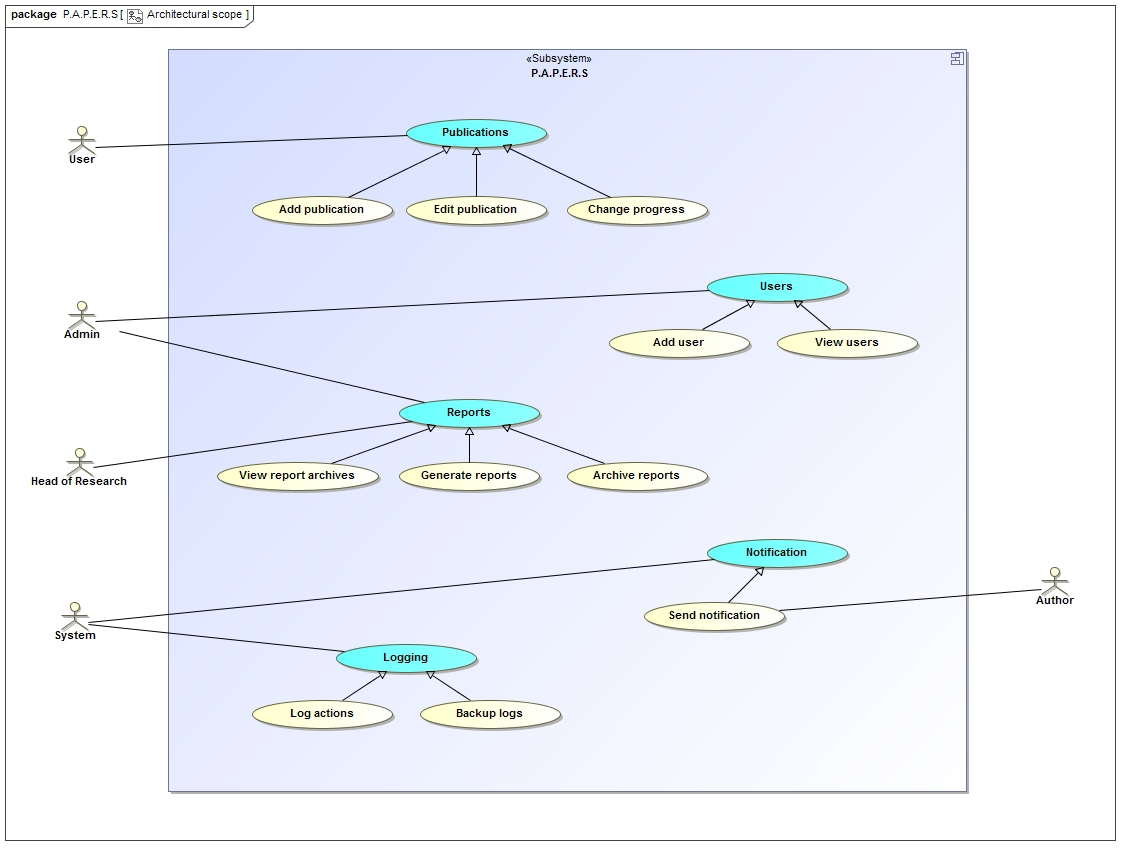
\includegraphics[width=\linewidth]{../Diagrams/Architectural Scope/Architectural scope.jpg}
		\caption{Architectural Scope - Use case for Architectural Scope (Further refined in use cases)}
	\end{figure}
	
	\par The system will be used to keep track of publications made for various research groups in the department, as well as keep track of the authors and the users in charge of things. From this we may later then generate reports on how various groups are doing as well as the department as a whole, and notify authors and users about upcoming deadlines and events.\\
	
	\par In the event of dealing with queries on database items such as users and publications, for example insertion and deletion, as well as viewing, the system must first validate that those items do or do not exist in said database. Once that is verified, the queries should be run and the result returned. On success the user should be notified, on failure an appropriate exception should be thrown. Persistence must be maintained throughout the database with very little fault tolerance.\\
	
	\par In dealing with reports, data being queried should be validated and the system should ensure that all queried data is recent and correct, halting any new additions during reporting. Reports should be properly archived for later retrieval and properly backed up regularly.\\
	
	\par In dealing with notifications, the system should ensure that all emails being used for every author does in fact exist and is a valid email. When sending this email, likely from the mail server at UP, the SMTP connection used must be ensured to be secured and the email should be sent through valid channels as to not appear as spam mail to other users. The system should also validate that it is using the latest deadline updates at all times.
	
	
	\cleardoublepage
	
	\subsection{Quality requirements}\label{subsec:quality}
	
	The core quality requirements for this system include in order:
	
	\begin{itemize}
		\item Cost
		\item Integrability,
		\item Security,
		\item Auditability,
		\item Reliability,
		\item Usability,
		\item Maintainability,
		\item Flexibility
		\item Performance, and
		\item Scalability. \newline
	\end{itemize}
	
	An in depth description of the various quality requirements: \newline
	
	\begin{itemize}
		\item Performance
		\begin{itemize}
			\item Performance in the system is of little worry as the system is not expected to grow to a large point in which it may slow down. The system should preferably be able to handle up to a hundred concurrent users at a time without major slow down effect and queries should be able to run within a matter of seconds.
		\end{itemize}
		\item Reliability
		\begin{itemize}
			\item The meta-data stored for each paper is required to be entirely correct at all times. To ensure this, we need to validate all possible input that can occur on the system in order to prevent any possible data inconsistencies. On the same note all data has to be persistent and remain in the database for the duration of the systems use, which means in all but the most extreme circumstances such as a database clean up for example, all entries must remain even if in a terminated state.
		\end{itemize}
		\item Scalability
		\begin{itemize}
			\item Scalability of this particular system is not of very particular importance. At the rate which the system will be used, chances of heavy fragmentation, data becoming too big or concurrency issues will be vary minimal.
		\end{itemize}
		\item Security
		\begin{itemize}
			\item Security is critical in the system as meta-data for unpublished papers can be sensitive information. Thus it is empirical that only authorised people have any access to the system at all. It is also vital to separate the concerns of each group from one another, allowing each group to only access the information from the groups they have access to. The Administrator should also be the only one allowed to make major changes to the system in anyway, and should be the only one authorised to make major persistence changes. 
		\end{itemize}
		\item Flexibility
		\begin{itemize}
			\item The system should be developed as to not be platform dependant or browser dependant in it's operation, allowing it to essentially be used from theoretically any device capable of an internet connection and HTML5, this includes iPhones which may still connect through safari as opposed to an iPhone application
			\item Flexibility may further be required in the event of change in units and venues for various existing conferences and journals, change in details for various users and authors registered on the system as well as flexibility for the addition or reduction of research groups.
		\end{itemize}
		\item Maintainability
		\begin{itemize}
			\item The system consists of a database which is required to stay consistent. To this end the system should contain well formatted documentation in order to properly maintain the system and ensure all data is in it's most consistent and reliable state.
		\end{itemize}
		\item Auditability
		\begin{itemize}
			\item All actions performed on the system should be audit-able via use of logging. A log entry should be created for each action such as adding or changing a publication for example. All actions performed in the system should be traceable to the user that performed them and possibly if so, where they performed it from in terms of IP as to have a form of accountability in the persistence of the meta-data.
		\end{itemize}
		\item Integrability
		\begin{itemize}
			\item The system should be easily integrable with the database system being used, allowing for simple queries in short amounts of time.
			\item The system should be integrable with a web front end that should allow users to easily and securely use all the features of the system that their authorisation level permits.
			\item The system should further be integrable with an Android front-end, which should allow for the exact same functionality of the web based front-end only designed ot be more mobile friendly.
		\end{itemize}
		\item Cost
		\begin{itemize}
			\item No proprietary software should be used in this system, and all licences for any software should be licensed under the open use policy.
		\end{itemize}
		\item Usability
		\begin{itemize}
			\item Users should easily be able to access the system securely from their most convenient location, either over their favourite web browser, the android application or via a mobile web page on their phone. All versions should allow full usage of all the features.
			\item Reports generated should be easily readable and allow for a logical and quick method of discerning various statistics from one another.
			\item Publications should be simple to view and easily distinguishable in type. One glance should allow a view of the most important details.
			\item Users should be easy to manage for the Administrator, allowing termination and reinstatement of users as well as addition of new ones to be a simple and streamlined process.
		\end{itemize}
	\end{itemize}
	
	\cleardoublepage
	
	\subsection{Integration and access channel requirements}\label{subsec:integration}
	
	\begin{itemize}
		\item The system must host a server to which API calls may be performed, to achieve this we use:
		\begin{itemize}
			\item Django (A Python based web framework allowing easy implementation of the MVC principal.)
			\item AngularJS (For easy unit testing functionality and dependency injection)
		\end{itemize}
		\item The system should make API calls via browser, the browser functionality and calling is done via:
		\begin{itemize}
			\item HTML5 (To ensure access to the latest and most stable versions of features)
			\item Javascript with a JQuery framework (For the functionality)
		\end{itemize}
		\item The system will require and android interface to interact with the API. To achieve this we make use of:
		\begin{itemize}
			\item JAVA (The standard language of every android application.)
			\item JQuery for mobile (A convenient method to manipulate data via JQuery on your android app.)
			\item Sencha touch (An HTML5 framework for Android.)
		\end{itemize}
		\item The system should be able to interact with the systems database, which will be hosted using:
		\begin{itemize}
			\item PostgreSQL (An open source relational database that integrates perfectly with the Django framework.)
		\end{itemize}
		\item The system should be able to send emails on a scheduled basis by sending mail from the CS mail server, for this we use:
		\begin{itemize}
			\item Django-sitemessage (A framework developed to allow easy scheduling of emails as well as the ability to retry an email on a failure.)\newline
		\end{itemize}
		
	\end{itemize}
	
	
	\begin{itemize}
		\item Protocols to be used include:
		\begin{itemize}
			\item HTTP
			\item SMTP
			\item TCP
		\end{itemize}
	\end{itemize}
	
	\cleardoublepage
	
	\subsection{Architectural constraints}\label{subsec:constraints}
	\begin{itemize}
		\item The system should be developed using only non-proprietary technologies.
		\item The system is to be developed for Linux based systems (Mostly Arch Linux) used by the Computer Science department, however preferably the system should run on any general use operating system.
		\item The system should be browser independent, thus the system should be accessed via any browser without issue, including but not limited to (Firefox, Chrome, Safari, Edge etc.)
		\item The system should be handled locally and should not rely on outside internet sources in order to function.
		\item The API created must be queried by both a web browser, as well as an Android application.
		\item The system created should allow for users to use the application via mobile, employing technologies such as bootstrap in order to keep it mobile friendly. This will always allow users of iOS and Windows mobile to access the system via channels such as Safari and Edge.
		\item The system is required to be concurrent and make use of concurrent methods specifically in it's functionality, allowing up to a minimum of a hundred concurrent users to be active at the same time
	\end{itemize}

	\section{Reference Architecture and frameworks}\label{sec: ReferencArchitecture}
In this section we will discuss the reference architecture and frameworks that will be used in the P.A.P.E.R system.
	\subsection{An object-relational mapper}\label{subsec: ORM}
	Object-relational mapper is a technique of converting data between incompatible systems by means of object orientated programming. For example the conversion of database attributes into a database object. This allow the interacting object-orientated language to manipulate this database object with ease, in essence the data can be presented in a way that any object is presented in that programming language.
	
	Django uses Object-relational mapping(ORM) with regards to its Model-View-Controller (MVC) model.
	The data models and a relational database (Model) are manipulated with the ORM strategy to interact with the databases.
		
	
	\subsubsection{Advantages}
	\begin{itemize}
	\item
	The advantage of using object-relational mappers with databases in particular is that joins aren't used that often as object types can be followed by means of referencing pointers. 
	\item
	Relationships are also established by means of pointers which can increase efficiency for complex data.
	\item
	This approach works well for large amounts of data, as the object can be manipulated easily for each field.
	\end{itemize}
	
	\subsubsection{Disadvantages}
	
	\begin{itemize}
	\item
	 Inefficient when used with small databases as objects will still be created which might be less efficient than a quick lookup of those particular fields. 
	\end{itemize}
	
	
	\clearpage
	
	\subsection{Application Server}\label{subsec: ApplicationServer}
	Software framework for web applications and a server to run the environment, is the principle that Application Server approach follows. An example of Application Server architecture framework is the Java EE framework. This architecture is based on the Layer model and Client-Server model and contains a service layer which is accessed by the developer.
	Django supports Java EE based Application Server.
	
	\subsubsection{Advantages}
	\begin{itemize}
	\item Scalability 
		\begin{itemize}
		\item Resources are allocated efficiently
		\item Objects reuse is ensured
		\end{itemize}
	\item Integrability
		\begin{itemize}
			\item Integrates well with REST
			\item Database integration is provided
		\end{itemize}
	\item Security
		\begin{itemize}
		\item Authentication and confidentiality is supported
		\end{itemize}
	\end{itemize}
	
	\subsubsection{Disadvantages}
	\begin{itemize}
	\item Uses a lot of system resources which might not necessarily be 
	\item Relies on server to be running at all times 
	\item Central point access can choke overall network's access to the server
	
	\end{itemize}
	%	\subsection{Service-Orientated Architecture }

	
	%	\subsubsection{Advantages}
	%	\subsubsection{Disadvantages}


\clearpage
\section{Reference Frameworks}\label{sec: RefFrameworks}


	\subsection{Django}\label{subsec: Django}
	Django is a web framework, written in Python which uses the Model-View-Controller architectural pattern, or MVC for short.
	Django's main aim is to provide a framework on which to build websites that are primarily based on complex databases.
	The use of Object-relational mapper in Django's MVC is described in \ref{subsec: ORM}. Django processes HTTP requests by means of a web templating system and regular-expression URL control (View and Controller).
	\\ \\
	\textbf{Django further includes:}
	\begin{itemize}
		\item Its own web server for developmental purposes.
		\item Form validation and storing of form data in database
		\item Caching framework with several cache methods
		\item Serialization system to produce and interpret XML and JSON representation of model instances.
		\item Python unit test framework
	\end{itemize}
	Django database support:
	\begin{itemize}
		\item PostgreSQL
		\item MySQL
		\item SQLite
		\item Oracle
		\item Microsoft SQL Server (through django-mssql)
	\end{itemize}
	Django can be used with:
	\begin{itemize}
		\item Python (Supported by default)
		\item JavaScript (through Swig)
		\item Ruby (through Liquid)
		\item Perl (through Template::Swig)
		\item PHP (Twig)
	\end{itemize}

	We prefer to use Django as it does have a slight learner curve, but will ease integrability with regards to our Android application.
	
	
	\subsection{Honorable Framework Mentions}
	\subsubsection{AngularJS}\label{subsubsec: AngularJS}
		Web-framework making use of client-side Model–View–Controller model. 
		AngularJS makes use of the MEAN stack for its front-end, consisting of MongoDB database, Express.js web application server framework, Angular.js itself, and Node.js runtime environment.
		We prefer to use a server side approach as this eases integrability and simplifies implementation.
	\subsubsection{Ruby on Rails}\label{subsubsec: Rails}
		Ruby based web-framework based on Ruby programming language. "Rails" uses a Model-View-Controller based model and emphasizes the use of JSON and XML for data transfer.
		Since Ruby has a high learning curve compared to Python for example, we prefer to use Django instead.
	\subsubsection{Zend Framework}\label{subsubsec: Zend}
	 Zend is an open source, object-oriented web application framework implemented in PHP 5. Zend supports multiple database systems and MVC is the preferred model of development.
	 Since Zend uses only Object-Orientated PHP5 we decided against this approach as the integration might be difficult for our Android Application.
	 \subsubsection{Bootstrap}\label{subsubsec: Bootstrap}
	 Bootstrap is a front-end framework for creating websites and applications. It is mainly used for interface development and design. Bootstrap can be used in HTML, CSS and JavaScript. 
	 We decided on a Server-side approach rather than a front-end approach such as Bootstrap.
	

\section{Technologies}

	For each of the following sections, all technologies we considered are listed.
	
	\subsection{Programming Languages}
			\subsubsection{Java}
				Java is a general purpose, high-level programming language developed by Sun Microsystems. It is concurrent, class based and object-oriented. It was specifically designed to have as few dependencies as possible.
				
				\begin{itemize}			
					\item Advantages:
						\begin{itemize}
							\item Easy to use
							\item Syntax is derived from C and C++
							\item Comprehensive documentation
						\end{itemize}
						
					\item Disadvantages:
						\begin{itemize}
							\item Memory Inefficient
						\end{itemize}
				\end{itemize}
				
			\subsubsection{JavaScript}
				JavaScript is a high-level programming language that is, alongside HTML and CSS, one of the three essential technologies that allow content production for the World Wide Web.
				
				\begin{itemize}
					\item Advantages:
						\begin{itemize}
							\item  Because JavaScript is client-side, there is no delay by having to wait for a server response
							\item Easy to learn and implement
						\end{itemize}
						
					\item Disadvantages:
						\begin{itemize}
							\item Security, the code being executed on the client-side is susceptible to malicious exploitation
						\end{itemize}
				\end{itemize}
				
			\subsubsection{Python}
				Python is a high-level programming language that emphasizes code readability.
			
				\begin{itemize}
					\item Advantages:
						\begin{itemize}
							\item Efficiency, Python allows a programmer to solve the same problem in fewer lines of code than in other languages such as Java
							\item Easy to read
						\end{itemize}
						
					\item Disadvantages:
						\begin{itemize}
							\item Syntax differs from conventional languages such as Java or C++, such as the omission of the semicolon
							\item Indentation dictates blocks of code, a single wrong indentation will produce undesired or unexpected results from your code
						\end{itemize}
				\end{itemize}
				
			\subsubsection{PHP}
				PHP (PHP: Hypertext Preprocessor) is a server-side scripting language designed for web development.
				
				\begin{itemize}
					\item Advantages:
						\begin{itemize}
							\item Works well with databases
							\item Popular, most problems encountered have already been solved by other developers
						\end{itemize}
						
					%\item Disadvantages:
					%	\begin{itemize}
					%		\item ?
					%	\end{itemize}
				\end{itemize}
				
			\subsubsection{C}
			
				\begin{itemize}
					\item Advantages:
						\begin{itemize}
							\item Fast run-time performance
						\end{itemize}
						
					\item Disadvantages:
						\begin{itemize}
							\item Low-level language, not ideal for applications or web development
						\end{itemize}
				\end{itemize}
				
			\subsubsection{C++}
			
				\begin{itemize}
					\item Advantages:
						\begin{itemize}
							\item Powerful language
							\item 
						\end{itemize}
						
					\item Disadvantages:
						\begin{itemize}
							\item No garbage collection, memory management has to be implemented by the programmer
							\item Complex language
						\end{itemize}
				\end{itemize}
				
			\subsubsection{HTML} %strictly speaking it is a markup language, but I think it fits with this section.
				HTML (HyperText Markup Language) is the standard markup language to create web pages. It dictates the content of a web page. Alongside JavaScript and CSS, it is one of the three essential technologies that allow content production for the World Wide Web.
				\begin{itemize}
					\item Advantages:
						\begin{itemize}
							\item Standardized, it is the standard markup language to create web pages
							\item Easy to learn
						\end{itemize}
					\item Disadvantages:
						\begin{itemize}
							\item Different web browsers may render the page differently
							\item Bland, it has limited styling capability.
						\end{itemize}
				\end{itemize}

		
	\subsection{Frameworks}
		\subsection{Ajax}
			AJAX (Asynchronous Javascript and XML) is a group of technologies used to create asynchronous web applications. It is used to change the content of a web page dynamically without having to reload the entire web page
			
		\subsection{AngularJS}
			Described in section \ref{subsubsec: AngularJS}
			
		\subsection{Bootstrap}
			Described in section \ref{subsubsec: Bootstrap}
			
		\subsection{Django}
			Described in detail in section \ref{subsec: Django}
			
	\subsection{Libraries}
			\subsubsection{jQuery}
			jQuery is a cross-platform JavaScript library designed to simplify client-side scripting. It is the most popular JavaScript library in use today
	
	\subsection{Protocols}
		All protocols listed below were discussed in section \ref{subsec:integration}
			\begin{itemize}
				\item LDAP (Lightweight Directory Access Protocol)
				\item HTTPS
				\item HTTP
				\item SMTP	
			\end{itemize}
	
	\subsection{Database Systems}
		The System will utilize a relational database and will use PostgreSQL to handle queries.
		
	\subsection{Operating Systems}
		The System will be created to primarily work on Linux as the entire Computer Department is running on Linux. The System will however be compatible with other operating systems such as Windows, Apple OS.
\end{document}
